% !TeX root = ../../main.tex
% The above "magic" comment allows us to compile only the main.tex file

\section{Experiment}
The GlueX experiment is objectively one of the best to ever do it 
\cite{ADHIKARI2021164807}. See figure~\ref{fig:schematic} for a schematic of the detector

\begin{figure}[h!]
    \centering
    % make sure to graphics are loaded in from the parent directory
    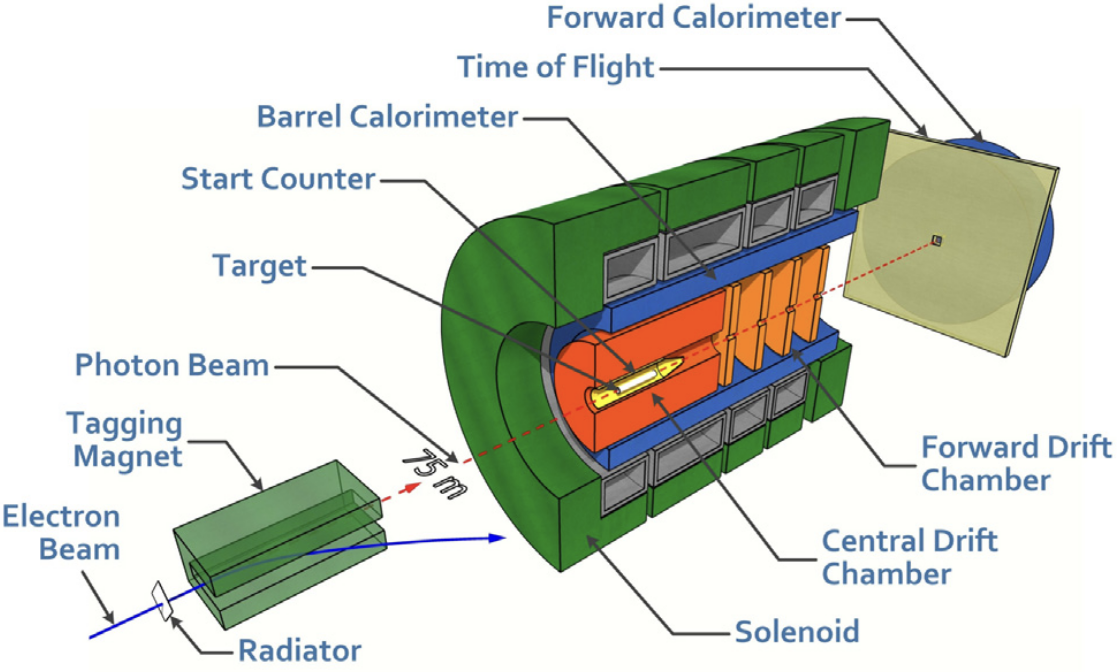
\includegraphics[width=0.8\textwidth]{sections/experiment/images/schematic.png}
    \caption{
        Drawing of the GlueX detector stationed in hall D at Jefferson Lab
        \cite{ADHIKARI2021164807}.
    }
    % labels are often given a prefix like "fig" for figure, "eq" for equation, etc. to 
    % indicate what is being labelled
    \label{fig:schematic} 
\end{figure}